Based on the implementation of the SOME/IP technology, the applications are run on the target hardware to realize the outcome. In this chapter, the results of several scenarios of the technology are presented and a brief overview of the troubleshooting guide is discussed.

\subsection{Server Application Output}
\begin{figure}[!htb]
	\centering
		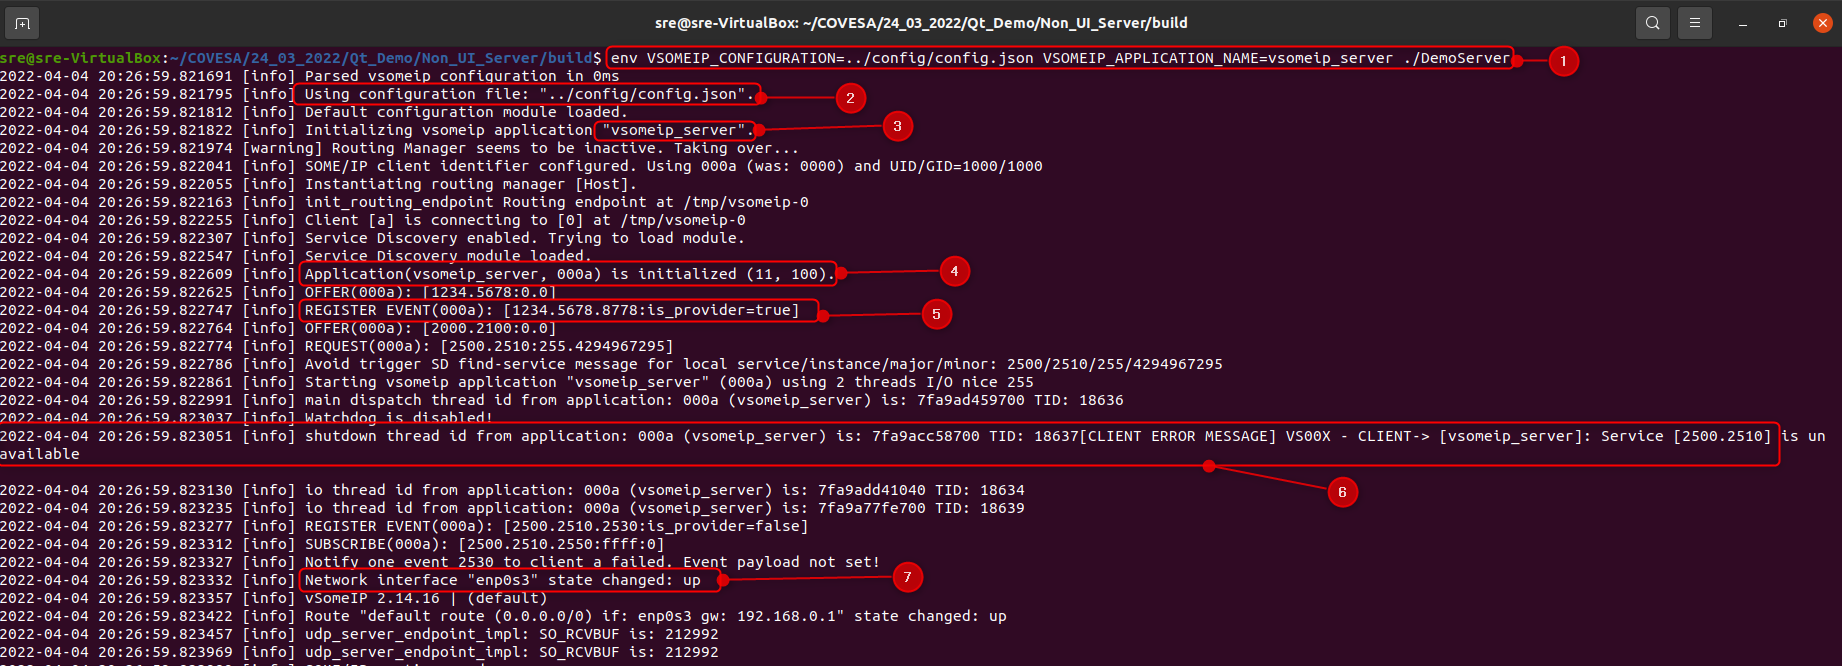
\includegraphics[width=1\textwidth]{images/res_server_eth0.png}
	\caption{Inter-ECU SOME/IP communication demonstration - Server}
	\label{fig:res_server_eth0}
\end{figure}


\subsection{Client Application Output}
\begin{figure}[!htb]
	\centering
		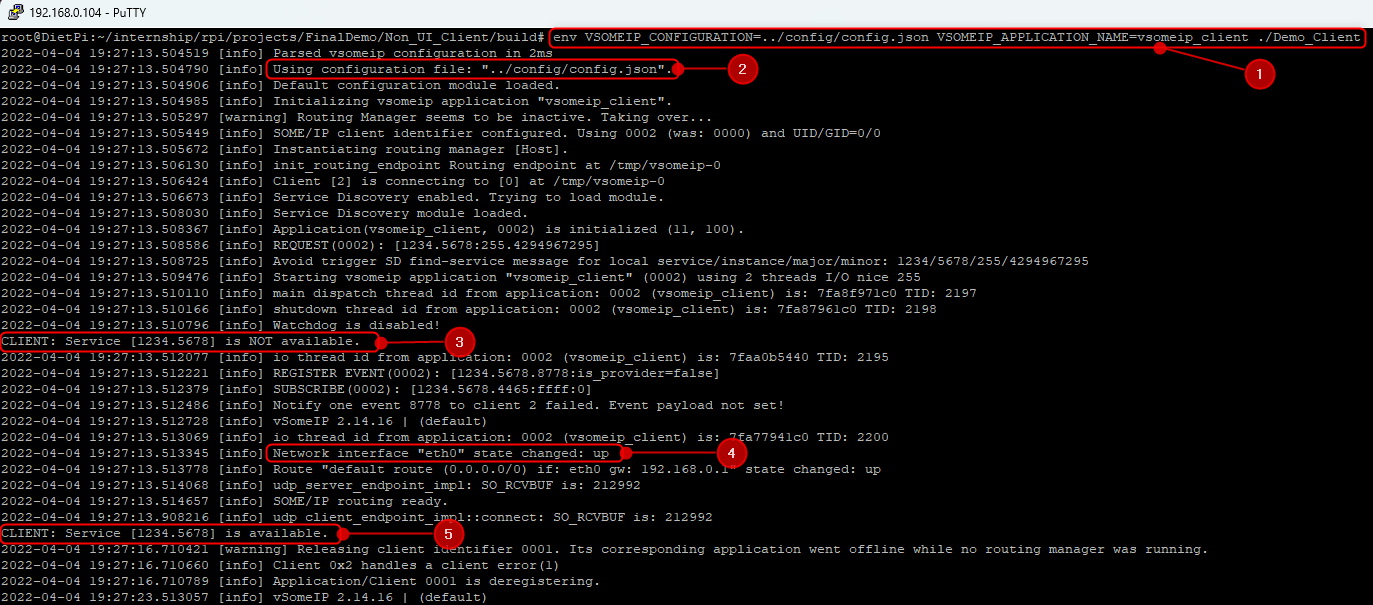
\includegraphics[width=1\textwidth]{images/res_client_eth0.png}
	\caption{Example of Inter-ECU SOME/IP communication - Client}
	\label{fig:res_client_eth0}
\end{figure}


\subsection{Troubleshooting guide}
Although user guide documentation for newer technologies is available, it is a challenge to set up and implement the technology. When it came to setting up the system and successfully running the applications on the target hardware during the development of the SOME/IP technology, there were many challenges. Some of these challenges were related to library and stack installation, which are well covered in the vsomeip stack user guide\cite{b_vsomeip_userguide}. However, several errors were discovered during the application's development and testing phases. Some of these errors can be caused by an incorrect method of implementing software code, while others can be caused by an improper configuration of the stack and applications.To avoid such issues in the future while developing SOME/IP-based applications, commonly encountered issues have been documented in the form of a troubleshooting guide. Each error message in this troubleshooting guide is assigned an error code, as well as the possible root cause and method for resolving the problem. Figure \ref{fig:troubleshooting_guide} depicts a section of the troubleshooting guide. The error messages displayed while running the applications are investigated, and the possible root cause and solutions are documented. This guide can be used by other developers who are using SOME/IP stacks provided by different vendors to try to replicate the issues using the demonstrator in order to better understand the problems.

\begin{figure}[!htb]
	\centering
		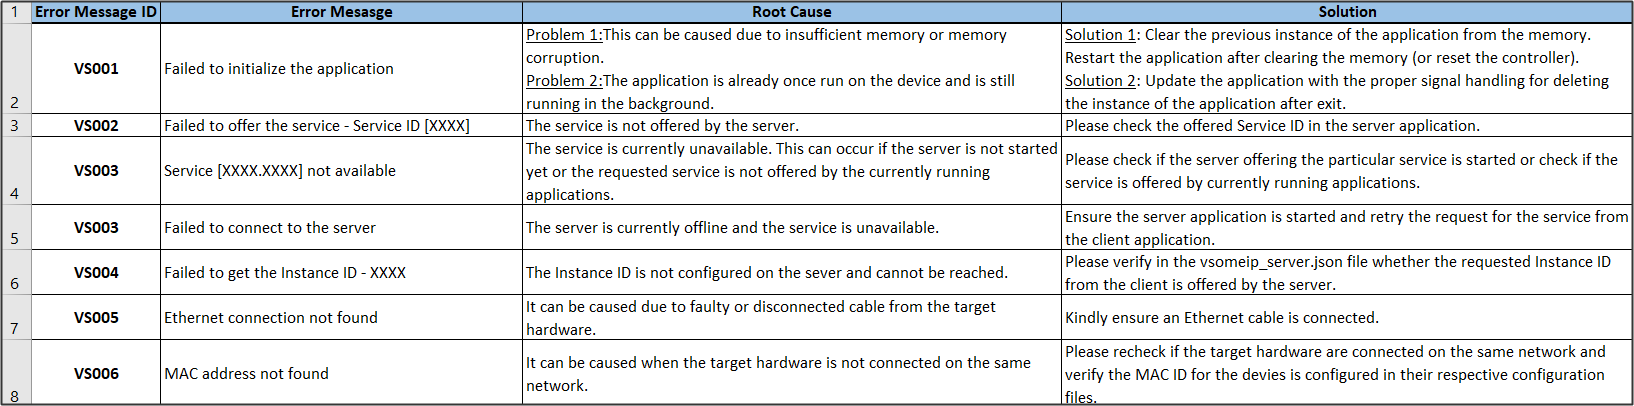
\includegraphics[width=1\textwidth]{images/troubleshooting_guide.png}
	\caption{SOME/IP troubleshooting guide}
	\label{fig:troubleshooting_guide}
\end{figure}
